% G07 - ECOM060 - Fase 2, Entrega final: instrumentacao nao ideal e seus efeitos no controle
% Compilar com: xelatex relatorio.tex (duas vezes)
\documentclass[10pt,a4paper]{article}
\usepackage[margin=1.6cm,top=1.4cm,bottom=1.6cm]{geometry}
\usepackage{fontspec}
\setmainfont{TeX Gyre Termes}
\usepackage{amsmath,amssymb}
\usepackage{graphicx,booktabs,tabularx,multirow,array,xcolor}
\usepackage[font=small,labelfont=bf,labelsep=period]{caption}
\usepackage{enumitem}
\usepackage{newunicodechar}
\usepackage{placeins}
\usepackage{tikz}
\usetikzlibrary{positioning,fit,backgrounds,arrows.meta}
\newunicodechar{Ω}{\ensuremath{\Omega}}
\newunicodechar{→}{\ensuremath{\to}}
\newunicodechar{×}{\ensuremath{\times}}
\newunicodechar{·}{\ensuremath{\cdot}}
\newunicodechar{≤}{\ensuremath{\le}}
\newunicodechar{≥}{\ensuremath{\ge}}
\newunicodechar{≈}{\ensuremath{\approx}}
\newunicodechar{≪}{\ensuremath{\ll}}
\newunicodechar{°}{\ensuremath{^\circ}}
\newunicodechar{µ}{\ensuremath{\mu}}
\newunicodechar{Δ}{\ensuremath{\Delta}}
\newunicodechar{σ}{\ensuremath{\sigma}}
\newunicodechar{−}{\ensuremath{-}}
\usepackage[hidelinks]{hyperref}
\renewcommand{\figurename}{Figura}
\renewcommand{\tablename}{Tabela}
\renewcommand{\refname}{Referências}
\setlist{nosep,leftmargin=*}
\setlength{\parskip}{2pt}
\newcolumntype{Y}{>{\raggedright\arraybackslash}X}
\makeatletter\let\inputtab\@@input\makeatother
\newcommand{\R}[1]{\FloatBarrier\par\medskip\noindent{\large\bfseries #1}\par\smallskip}
\newcommand{\pend}{\textcolor{red}{[captura pendente]}}
\emergencystretch=3em\sloppy
\begin{document}
\begin{center}
{\Large\bfseries Instrumentação não ideal e seus efeitos no controle de corrente do motor BLDC MOONS' R42BLD30L3}\\[2pt]
Grupo G07 — Fase 2, Entrega final — ECOM060 Instrumentação Eletrônica (UFAL, 2026.2)\\[4pt]
\begin{tabular}{ll}\toprule Nome completo & Matrícula\\\midrule
Nícolas De Almeida Souza & 23111883\\ Lucas Momesso Alves & 22112804\\ Cláudio Henrique da Costa Santos & 20211850\\\bottomrule\end{tabular}
\end{center}

\noindent\textbf{Resumo.} O mesmo controlador de corrente que atende a todos os critérios com medição ideal deixa o motor 23 mA abaixo da referência e viola a acomodação (4,8 ms contra 3 ms) quando passa a usar a medição real com o sensor Hall ACS712. A diferença vem sobretudo do ruído retificado pelo processamento, e o ponto mais frágil é o desvio de zero: o erro estacionário deixa de ser atendido com 1,4 mV de zero não compensado ou com 15 mV de ruído. A autocalibração do zero (limite de 1,4 para 97 mV) e a escolha da fase pela posição (limite do ruído de 15 para 78 mV; erro de 23 para 11 mA) recuperam o desempenho; a correção calculada do filtro RC não funcionou, e o filtro passa a ser uma exigência de projeto ($f_c$ ≥ 1,2 kHz).

\noindent Este relatório consolida as Entregas 01 a 04 da Fase 2 e avalia como as características não ideais da medição da corrente de fase alteram o controle de corrente do motor. Cada seção corresponde a um item do Quadro 1 da orientação. Todos os ensaios usam um único modelo (\texttt{modelo\_final.tse}) e um único painel do HIL SCADA (\texttt{painel\_final.cus}); a versão do software, os arquivos e os passos de cada captura estão no \texttt{README.md} da pasta \texttt{simulacao}. A Entrega 01 \cite{e01} fornece o modelo e os parâmetros do motor (item 1), de onde sai a demanda de medição (item 2); as Entregas 02 a 04 \cite{e02,e03,e04} fornecem o equivalente, a instrumentação e o controle. Figuras e tabelas dessas entregas foram reaproveitadas com os mesmos valores.

%======================================================================
\R{1. Sistema e equivalente}
O sistema original é um motor BLDC MOONS' R42BLD30L3 \cite{moons} (42 mm, 36 V, 30 W, 8 polos, sensores Hall a 120°) acionando um ventilador, alimentado por um inversor trifásico seis-passos com PWM de 10 kHz e razão cíclica $d$ (Fig.~\ref{fig:sis}). A Tab.~\ref{tab:e01} resume a caracterização da E01 \cite{e01}, de onde saem a demanda de medição (item 2) e os critérios de controle (item 5). No equivalente elétrico (Fig.~\ref{fig:circ}, E02 \cite{e02}), a parte elétrica fica em 1:1 e a mecânica vira um circuito pela analogia força–tensão (Tab.~\ref{tab:analog}).

\begin{figure}[!htbp]\centering
\begin{minipage}[c]{.6\textwidth}\centering\scriptsize\setlength{\tabcolsep}{3pt}
\captionof{table}{Sistema original (E01 e catálogo \cite{moons}).}\label{tab:e01}
\begin{tabular}{@{}p{1.9cm}p{3.1cm}p{5.3cm}@{}}\toprule
Grandeza & Valor & Uso\\\midrule
$V_s$; $R_s$; $L_s$ & 36 V; 1,60 $\Omega$; 1,90 mH & $L_s/R_s$ = 1,19 ms; projeto do PI\\
$k$; $J$; $B$ & 0,048 N·m/A; 3,3 g·cm²; 10$^{-6}$ N·m·s & $T_e = k\,i$: medir corrente é medir torque\\
Ponto nominal & 4000 rpm; 1,675 A & $f_e = pn/60$ = 267 Hz; banda 13$f_e$ ≈ 3,5 kHz\\
Pico; partida & 5 A (catálogo); 6,4 A & faixa do sensor ±10 A\\
Malha de velocidade & acomoda em ≈11 ms & malha de corrente ≤ 3 ms\\\bottomrule
\end{tabular}
\end{minipage}\hfill
\begin{minipage}[c]{.37\textwidth}\centering
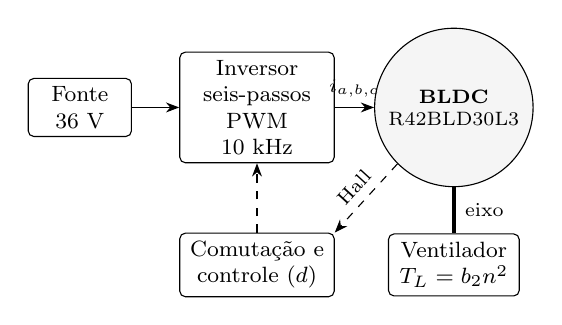
\begin{tikzpicture}[font=\footnotesize, >=Stealth, bx/.style={draw, rounded corners=2pt, align=center, fill=white, inner sep=3pt}]
\node[bx, text width=1.1cm] (vs) at (0,0) {Fonte\\36 V};
\node[bx, text width=1.75cm] (inv) at (2.25,0) {Inversor\\seis-passos\\PWM 10 kHz};
\node[draw, circle, minimum size=1.45cm, align=center, fill=gray!8, font=\scriptsize] (m) at (4.75,0) {\textbf{BLDC}\\R42BLD30L3};
\node[bx, text width=1.75cm] (lg) at (2.25,-2.0) {Comutação e controle ($d$)};
\node[bx, text width=1.45cm] (fan) at (4.75,-2.0) {Ventilador\\$T_L = b_2 n^2$};
\draw[->] (vs) -- (inv);
\draw[->] (inv) -- node[above, font=\scriptsize]{$i_{a,b,c}$} (m);
\draw[line width=1.4pt] (m.south) -- node[right, font=\scriptsize]{eixo} (fan.north);
\draw[->, dashed] (m.south west) -- node[above, sloped, font=\scriptsize]{Hall} (lg.north east);
\draw[->, dashed] (lg) -- (inv);
\end{tikzpicture}

\captionof{figure}{Sistema original. Sem o motor físico, o grupo o representa por este diagrama.}\label{fig:sis}
\end{minipage}
\end{figure}

\begin{figure}[!htbp]\centering
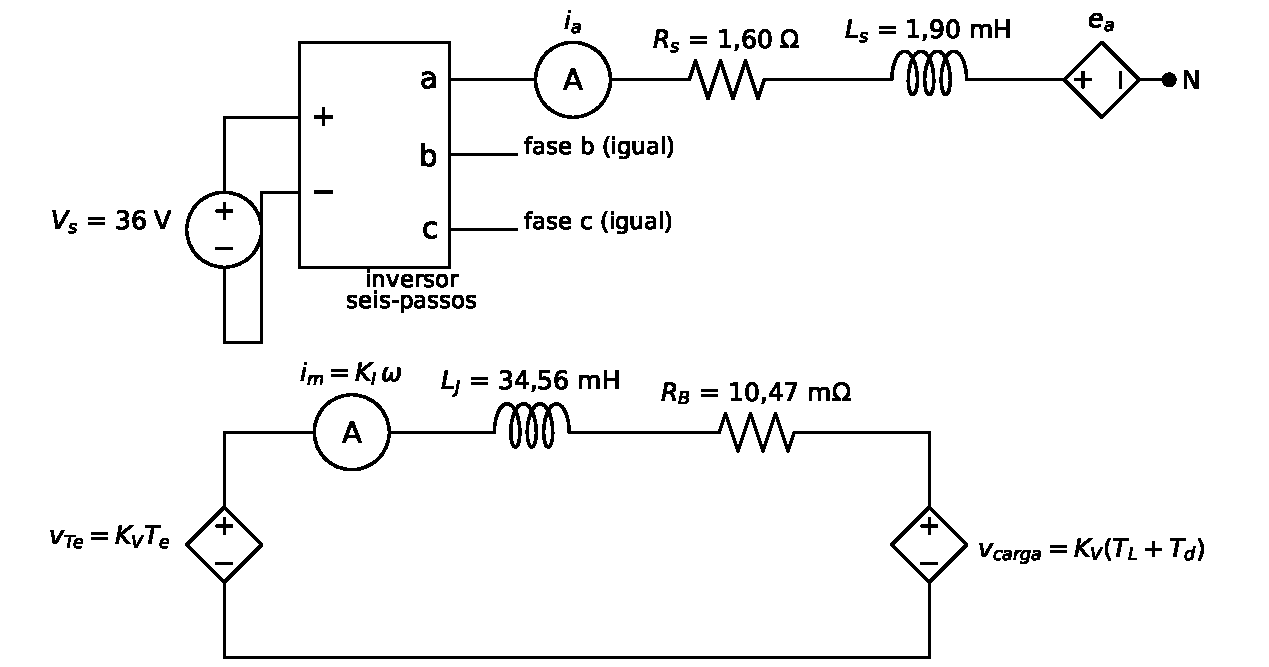
\includegraphics[width=.84\textwidth]{figuras/fig_circuito.pdf}
\caption{Circuito equivalente no TyphoonSim. Em cima, a fase $a$ do motor em 1:1 ($b$ e $c$ iguais); embaixo, a malha mecânica. Uma \texttt{C function} de acoplamento lê $i_a$, $i_b$, $i_c$ e $i_m$ e escreve a FCEM $e_x$ e as tensões $v_{Te}$ e $v_{carga}$.}\label{fig:circ}
\end{figure}

\begin{table}[!htbp]\centering\footnotesize
\caption{Analogia força–tensão e escalas ($K_V$ = 100 V/(N·m); $K_I$ = 9,549$\times10^{-3}$ A·s/rad, ou seja 1 A = 1000 rpm; tempo em 1:1).}\label{tab:analog}
\begin{tabularx}{\textwidth}{p{3.9cm}p{3.6cm}p{3.6cm}Y}\toprule
Grandeza original & Grandeza no circuito & Escala & Valor / elemento\\\midrule
torque $T$; velocidade $\omega$ & tensão $v$; corrente $i_m$ & $v = K_V T$; $i_m = K_I\omega$ & 1 V = 10 mN·m; 4000 rpm = 4 A\\
inércia $J$; atrito $B$ & indutor $L_J$; resistor $R_B$ & $\times K_V/K_I$ & 34,56 mH; 10,47 m$\Omega$\\
$T_e$, carga $T_L = b_2 n^2$, pulso $T_d$ & fontes de tensão controladas & $K_V$ & \texttt{G07\_V\_Te}, \texttt{G07\_V\_carga}\\
corrente de fase, $R_s$, $L_s$, $V_s$ & os mesmos & 1:1 & 1,60 $\Omega$; 1,90 mH; 36 V\\\bottomrule
\end{tabularx}
\end{table}

\noindent\textbf{Equação comum aos dois domínios.} Dividindo a malha mecânica do circuito por $K_V$ e usando $i_m = K_I\omega$ (os polos e o ganho estático são os da E01; a validação no Virtual HIL deu 19 de 22 itens dentro do critério \cite{e02}):
\begin{equation}
\underbrace{L_J\frac{di_m}{dt} + R_B\,i_m = v_{Te} - v_{carga}}_{\text{circuito}}
\quad\Longleftrightarrow\quad
\underbrace{J\frac{d\omega}{dt} + B\,\omega = T_e - T_L - T_d}_{\text{motor}},
\qquad v_x = R_s i_x + L_s\frac{di_x}{dt} + e_x \ \text{(nos dois)}.
\end{equation}

%======================================================================
\R{2. Sensor e localização da instrumentação}
\textbf{Grandeza e sensor.} A grandeza medida é a \textbf{corrente de fase} do motor, que produz o torque ($T_e = k\,i$, com $k$ = 0,048 N·m/A). A demanda (Tab.~\ref{tab:dem}) vem do item 1 (Tab.~\ref{tab:e01}) e da corrente simulada: partida de 6,4 A; frequência elétrica de até 267 Hz no ponto nominal de 4000 rpm (244 Hz no ensaio de malha aberta, ≈247 Hz na malha fechada com 1,5 A), com a forma de 120° exigindo harmônicas até a 13.ª (3,5 kHz); e ondulação de PWM de 0,68 A p-p em 10 kHz. O sensor escolhido é o de \textbf{efeito Hall} Allegro ACS712ELCTR-20A-T \cite{acs712} (Aguirre, Seções 7.6 e 8.2.1 \cite{aguirre}), mais simples de ligar ao inversor que o shunt: é isolado do barramento e já entrega uma tensão proporcional à corrente ($V_Q + S\,i$, com $V_Q$ = 2,5 V e $S$ = 100 mV/A), sem amplificador diferencial. A versão de 20 A cobre a partida (a de 5 A saturaria) e sua banda de 80 kHz é 23 vezes a pedida.

\begin{table}[!htbp]\centering\footnotesize
\caption{Demanda de medição (do item 1 e da E03) e o que o ACS712-20A com a cadeia oferece.}\label{tab:dem}
\begin{tabularx}{\textwidth}{p{2.3cm}p{2.7cm}Y p{3.2cm}}\toprule
Grandeza & Requisito & Origem & ACS712 + cadeia\\\midrule
Faixa & ±10 A & partida de 6,4 A (acima do pico de catálogo, 5 A), com margem & ±25 A (0 a 5 V)\\
Banda & 0 a 3,5 kHz & 13.ª harmônica de $f_e$ = 267 Hz (4000 rpm); 99,8 \% da potência abaixo de 3,5 kHz & 80 kHz (sensor); ≈4,4 kHz depois da média\\
Resolução & ≤ 40 mA & 1/5 do $\Delta i$ eficaz do pulso de carga (0,21 A) & 12,2 mA (ADC de 12 bits)\\
Incerteza & viés ≤ 25 mA; aleatória ≤ 70 mA rms & 2 \% de 1,14 A eficazes (erro de torque de 2 \%) & viés ≤ 2 mA; 58 mA rms\\
Atraso & ≤ 100 µs & um período de PWM & 60 µs\\\bottomrule
\end{tabularx}
\end{table}

\textbf{Onde se mede.} O ramo medido é o de cada fase do circuito equivalente: os amperímetros ideais \texttt{G07\_iS} e \texttt{G07\_iSb} (\texttt{core/Current Measurement}) estão em série com $R_s$, $L_s$ e $e_x$ das fases $a$ e $b$ (Fig.~\ref{fig:circ}). Como a parte elétrica do equivalente está em 1:1, a corrente desse ramo \emph{é} a corrente do enrolamento, em ampères: a escala da analogia para essa grandeza é 1 (se fosse medido o torque, em $v_{Te}$, a escala seria $K_V$). A fase $c$ não tem sensor: $i_c = -(i_a + i_b)$, como nos acionamentos comerciais. O sensor converte A em V com $S$ = 100 mV/A, e cada característica atua sobre a tensão de saída (ou, no caso da sensibilidade, sobre o ganho), na unidade do sensor; o processamento devolve o valor em ampères.

\textbf{Carregamento (Seção 3.4).} O ACS712 insere 1,2 m$\Omega$ no ramo, contra 1,6 $\Omega$ de $R_s$ (3,2 $\Omega$ entre fases): a corrente muda menos de 0,04 \%, abaixo de qualquer outro efeito. Por isso o carregamento não foi inserido no circuito, e o sensor entra só como pós-processamento da leitura do amperímetro ideal. O campo do condutor primário também não age sobre o motor.

\begin{figure}[!p]\centering
\resizebox{\textwidth}{!}{% Figura 1 da orientacao, preenchida com os blocos do modelo_final.tse (G07) - versao vertical
\begin{tikzpicture}[font=\small, >=Stealth, line width=0.6pt,
  bx/.style={draw, rounded corners=2pt, align=center, fill=white, inner sep=4pt, text width=#1},
  bx/.default=4.2cm, ins/.style={bx=#1, fill=gray!10}, ins/.default=4.2cm,
  d/.style={font=\footnotesize}]
\node[bx=4.6cm] (pl) at (6.5,0) {\textbf{Planta} (equivalente elétrico)\\[1pt]{\footnotesize fases \texttt{G07\_Rs/Ls/e\_x};\\ malha mecânica \texttt{G07\_L\_J}, \texttt{G07\_R\_B}}};
\node[bx=4.6cm] (pp) at (6.5,-2.1) {\textbf{Ponta de prova ideal}\\[1pt]{\footnotesize amperímetros \texttt{G07\_iS} e \texttt{G07\_iSb} em série com as fases $a$ e $b$}};
\node[ins] (se) at (3.9,-4.9) {\textbf{Sensor} ACS712-20A\\[1pt]{\footnotesize \texttt{S1} sensibilidade · \texttt{S2} zero\\ \texttt{S3} banda · \texttt{S4} ruído}};
\node[ins] (co) at (3.9,-7.2) {\textbf{Condicionamento}\\[1pt]{\footnotesize \texttt{C1} filtro RC (15 kHz)\\ \texttt{C2} ADC (12 bits, 20 kS/s)}};
\node[ins] (pr) at (3.9,-9.6) {\textbf{Processamento e compensação}\\[1pt]{\footnotesize \texttt{P1}: correção calculada, média, autocalibração\\ \texttt{CL\_realimentacao}: módulo ou fase pela posição; correção do RC}};
\begin{scope}[on background layer]
\node[draw=gray, dashed, rounded corners, fill=gray!4, fit=(se)(co)(pr), inner sep=6pt] (box) {};
\end{scope}
\node[d, font=\footnotesize\bfseries, align=center, anchor=north] at (box.south) {Aqui atua a instrumentação (fases $a$ e $b$)};
\node[bx=2.9cm] (es) at (-0.9,-7.2) {\textbf{Entradas espúrias}\\[1pt]{\footnotesize temperatura \texttt{G07\_T} (60 °C)\\ ruído \texttt{G07\_ruido}}};
\node[bx=3.4cm] (id) at (10.4,-7.2) {\textbf{Caminho ideal}\\ ganho 1\\[1pt]{\footnotesize \texttt{G07\_Med\_ideal}; $i_{pl}$ em \texttt{G07\_CL\_realimentacao}}};
\node[bx=3.8cm] (sel) at (7.0,-12.6) {\textbf{Seletor ideal/real}\\[1pt]{\footnotesize caixa \texttt{G07\_fb\_real}}};
\node[bx=3.2cm] (rf) at (1.2,-14.9) {\textbf{Referência} $r$\\[1pt]{\footnotesize \texttt{G07\_CL\_referencia}}};
\node[bx=3.8cm] (ct) at (7.0,-14.9) {\textbf{Controlador}\\[1pt]{\footnotesize \texttt{G07\_CL\_erro} (Sum) e \texttt{G07\_CL\_PI} (PI)}};
\node[bx=3.0cm] (at) at (12.4,-14.9) {\textbf{Atuador}\\[1pt]{\footnotesize \texttt{G07\_Seletor\_duty} e inversor (PWM 10 kHz)}};
% ligacoes
\draw[->] (pl) -- node[right, d]{$y_{real}$ ($i_a$, $i_b$)} (pp);
\draw[->] (pp.south) -- ++(0,-0.45) -| (se.north);
\draw[->] (pp.south) -- ++(0,-0.45) -| (id.north);
\draw[->] (se) -- (co); \draw[->] (co) -- (pr);
\draw[->] (es) -- (es -| box.west);
\draw[->] ([yshift=-6mm]pr.south) |- ([yshift=2mm]sel.west) node[pos=0.75, above, d]{$y_{med}$};
\draw[->] (id.south) |- ([yshift=2mm]sel.east) node[pos=0.75, above, d]{$y_{ideal}$};
\draw[->] (sel) -- (ct);
\draw[->] (rf) -- node[above, d]{$r$} (ct);
\draw[->] (ct) -- node[above, d]{$u$} (at);
\draw[->] (at.north) |- node[pos=0.75, above, d]{razão cíclica $d$} (pl.east);
\draw[->, dashed] (se.west) -- ++(-1.25,0) |- ([yshift=-2mm]pl.west) node[pos=0.75, above, d, align=center, text width=3.4cm]{carregamento: 1,2 m$\Omega$ ≪ 1,6 $\Omega$\\(< 0,04 \%), desprezado};
\end{tikzpicture}
}
\caption{Figura 1 da orientação preenchida com os blocos do \texttt{modelo\_final.tse}. As duas cadeias (fases $a$ e $b$) são iguais, com geradores de ruído independentes. O seletor, as compensações e as intensidades das características são caixas do HIL SCADA, ajustáveis com o modelo rodando.}\label{fig:f1}
\end{figure}

%======================================================================
\R{3. Características do instrumento}
A Tab.~\ref{tab:car} traz as características modeladas: quatro estáticas, três dinâmicas, duas entradas espúrias e quatro originadas no condicionamento ou no processamento. Cada uma é um bloco \texttt{C function} do caminho real (Fig.~\ref{fig:f1}), com a intensidade ajustada por uma caixa do SCADA (0 desliga; $T$ = 25 °C anula as derivas). Os blocos nativos de ganho, filtro e quantização têm parâmetros fixos na compilação e não permitem esse ajuste ao vivo; o código está em \texttt{simulacao/codigo\_c\_functions.md}.

\begin{table}[!htbp]\centering\scriptsize\setlength{\tabcolsep}{3pt}
\caption{Características do instrumento: definição (seção de Aguirre \cite{aguirre}), valor com fonte, modelo matemático (bloco) e efeito esperado na leitura da corrente da fase $a$ (regime do ensaio de degrau, 1,14 A eficazes).}\label{tab:car}
\begin{tabularx}{\textwidth}{p{2.3cm}p{3.2cm}p{2.9cm}p{3.6cm}Y}\toprule
Característica (tipo) & Definição (livro) & Valor e fonte & Modelo (bloco) & Efeito esperado\\\midrule
Sensibilidade e erro de sensibilidade (estática) & variação da saída por unidade de entrada; o erro é o afastamento do valor nominal (3.3.1, 3.3.8) & $S$ = 100 mV/A; $e_S$ = +1,5 \% (erro total $E_{TOT}$ do datasheet, pior caso) & $v = S(1+e_S)\,i$ (\texttt{S1}) & leitura 1,5 \% maior: 15,5 mA rms; sem viés na média de uma corrente alternada\\
Desvio de zero (estática) & saída com entrada nula diferente do valor nominal (3.3.8) & $e_Q$ = +10 mV (estimativa declarada, dentro de $E_{TOT}$) & $v = V_Q + e_Q + S\,i$ (\texttt{S2}) & +100 mA constantes sem correção\\
Temperatura (entrada espúria: modificante e interferente) & altera a sensibilidade (modificante) e desloca o zero (interferente) (2.4) & $T$ = 60 °C (estimativa: placa do inversor); $-$0,07 mV/°C e $-$0,004 mV/A/°C (datasheet) & $\Delta V_Q = -0{,}07(T-25)$ mV; $\Delta S = -0{,}004(T-25)$ mV/A (\texttt{S1}, \texttt{S2}) & zero $-$2,45 mV ($-$24,5 mA); ganho $-$0,14 \%\\
Resposta dinâmica (dinâmica) & sistema de 1.ª ordem: constante de tempo e banda (4.2.2) & 80 kHz, subida de 3,5 µs (datasheet) & $H_s = 1/(1+s/\omega_s)$, Euler regressivo a 5 µs (\texttt{S3}) & atraso de 2 µs; $-$0,1 \% em 3,5 kHz; 8 mA rms sobre a ondulação\\
Ruído (entrada espúria aleatória) & sinal aleatório somado à saída; caracterizado pelo valor rms e pela banda (5.4) & 10 mV rms em 100 kHz (de 11 mV p-p em 2 kHz do datasheet) & $v \mathrel{+}= \sigma_v\,n$, $n$ gaussiana (Park–Miller, soma de 6 uniformes) (\texttt{S4}) & 100 mA rms brutos; ≈31 mA na média por período (Tab.~\ref{tab:contr})\\
Faixa (estática) & intervalo de entrada medido sem saturar (3.3.6) & 0 a 5 V = ±25 A (alimentação de 5 V) & saturação no ADC (\texttt{C2}) & não exercitada: pico de 6,4 A\\
Filtro anti-aliasing RC (\textbf{circuito auxiliar}, dinâmica) & filtro passa-baixas de 1.ª ordem (6.2.1) & $f_c$ = 15 kHz (projeto) & $H_{RC} = 1/(1+s/\omega_c)$ (\texttt{C1}) & atraso de 10,6 µs; $-$2,6 \% em 3,5 kHz; $|H(f_e)|$ = 0,9999. Com $f_c$ perto de $f_e$, a leitura cai para $|H(f_e)|\,i$\\
Amostragem e quantização (\textbf{circuito auxiliar}, estática e dinâmica) & resolução: menor variação detectável (3.3.2); amostragem e retenção & 12 bits em 5 V; 20 kS/s síncrono com o PWM (projeto) & retém a amostra por 50 µs; $q$ = 5 V/2$^{12}$ = 1,22 mV = 12,2 mA (\texttt{C2}) & erro de quantização $q/\sqrt{12}$ = 3,5 mA rms; parte do atraso\\
Média por período de PWM (\textbf{processamento}, dinâmica) & filtro digital de média móvel (6.2.2) & 100 µs = 2 amostras (projeto) & $|H| = |\sin(\pi fT)/(\pi fT)|$, zero em 10 kHz (\texttt{P1}) & remove a ondulação de 10 kHz; banda de $-$3 dB ≈ 4,4 kHz; atraso ≈ 50 µs (60 µs na cadeia)\\
Correção calculada (\textbf{processamento}) & compensação por um modelo da entrada espúria (2.5.3) & zero, ganho e temperatura calibrados & $i = (v - V_{Qc})/S_c$ (\texttt{P1}) & remove o zero, o erro de ganho e a deriva, se a calibração estiver certa\\
Módulo das três correntes (\textbf{processamento}, não linear) & retificação de um sinal aleatório: $E|n| = \sigma\sqrt{2/\pi}$ (5.4) & $i = (|i_a|+|i_b|+|i_c|)/2$ (E04) & a fase que não conduz só tem ruído e soma $|n|$ (\texttt{G07\_CL\_realimentacao}) & viés de 0,455 $\sigma_f$ ≈ +14 mA na medida, só visível em malha fechada\\\bottomrule
\end{tabularx}
\end{table}

As três exigidas pela orientação: a \textbf{estática} é o desvio de zero (com a sensibilidade); a \textbf{dinâmica} é a resposta de 1.ª ordem do sensor (com o filtro RC e a média); a \textbf{entrada espúria} é a temperatura (com o ruído). As originadas em circuito auxiliar ou processamento são o filtro RC, o ADC, a média e o módulo. Não foram incluídas a não linearidade e a histerese, desprezíveis no datasheet frente às demais, e o acoplamento de campos externos, que depende da montagem e não tem valor publicado.

%======================================================================
\R{4. Efeito em malha aberta}
Em malha aberta (o controle usa a razão cíclica fixa da E01), a leitura ideal coincide com a corrente verdadeira em todas as amostras. Cada bloco do caminho real também calcula a leitura com \emph{só a sua} característica (saídas \texttt{G07\_iso\_*}), o que separa as contribuições numa única captura (Fig.~\ref{fig:contr} e Tab.~\ref{tab:contr}).

\begin{figure}[!htbp]\centering
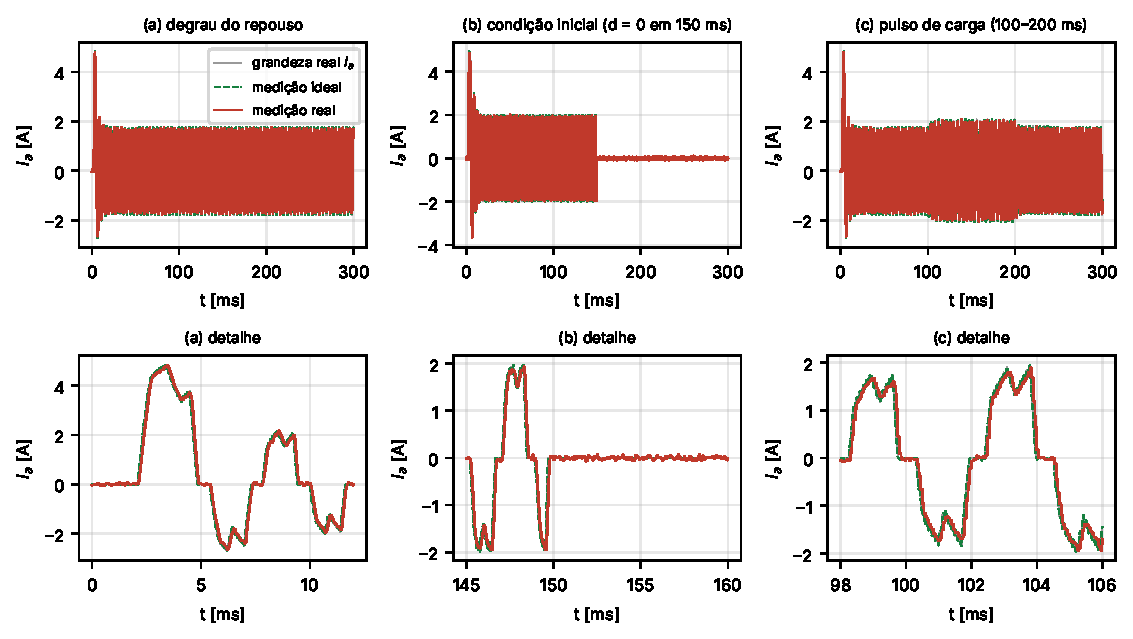
\includegraphics[width=\textwidth]{figuras/fig_ensaios.pdf}
\caption{Leitura ideal × real nos três ensaios de malha aberta (VHIL, preset \texttt{Item4\_malha\_aberta}), com a cadeia real completa.}\label{fig:ens}
\end{figure}

\begin{figure}[!htbp]\centering
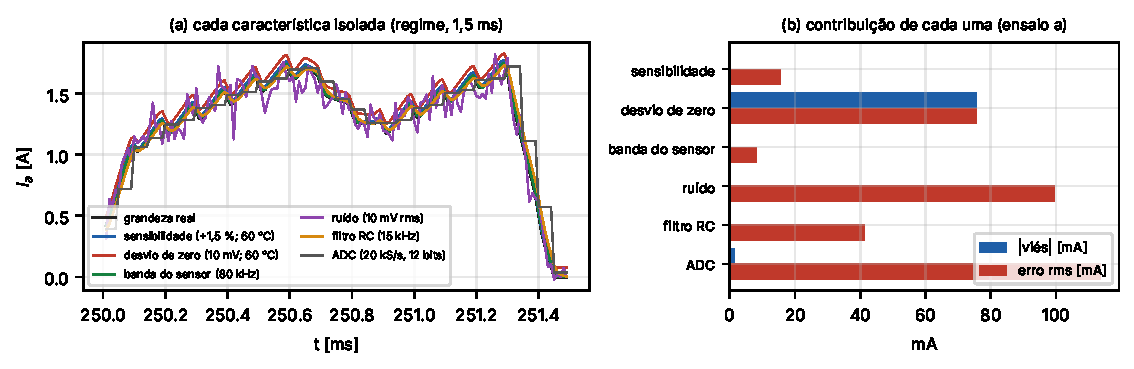
\includegraphics[width=\textwidth]{figuras/fig_contribuicoes.pdf}
\caption{(a) Leitura com cada característica ligada isoladamente, em regime. (b) Contribuição de cada uma para a diferença entre leitura e grandeza real.}\label{fig:contr}
\end{figure}

\begin{table}[!htbp]\centering\footnotesize
\caption{Contribuição de cada característica isolada (ensaio de degrau, 200–300 ms): viés, erro rms contra a corrente instantânea e erro rms das médias por período de PWM.}\label{tab:contr}
\begin{tabular}{lrrrl}\toprule
Característica (só ela ligada) & Viés [mA] & Erro rms [mA] & Erro rms na média [mA] & Explicação\\\midrule
\inputtab tabelas/tab_item4_contr.tex \bottomrule
\end{tabular}
\end{table}

\textbf{Leitura.} O \textbf{desvio de zero} é a única característica que desloca a média: 75,5 mA = $(10 - 0{,}07\cdot35)$ mV $/S$, como previsto na Tab.~\ref{tab:car}. Ruído, ADC e filtro RC espalham a leitura (erro rms de 30 a 76 mA na média), mas não a deslocam; a sensibilidade só muda a escala (+1,5 \%) e a banda do sensor quase não aparece. Com a cadeia completa e a correção calculada, o viés fica em 0,5 a 2 mA, o erro rms em 58 mA (atraso de 60 µs descontado) e, com a corrente nula, a leitura marca 1,2 mA, contra 75,5 mA sem a correção. A medição atende à demanda da Tab.~\ref{tab:dem}.

%======================================================================
\R{5. Controle com instrumento ideal}
\textbf{Malha e critérios.} A malha fechada sobre a corrente medida é a malha de corrente (torque) do acionamento, interna à de velocidade do ventilador. A grandeza controlada é a corrente do par em condução, $(|i_a|+|i_b|+|i_c|)/2$, e a mesma expressão sobre as correntes verdadeiras dá a \emph{grandeza real da planta}. Os critérios estão na Tab.~\ref{tab:spec}; as métricas usam a média de dois intervalos de comutação (≈1,3 ms), porque a corrente tem uma ondulação física de ±0,3 A a cada comutação e é o valor médio que produz torque.

\begin{table}[!htbp]\centering\footnotesize
\caption{Critérios de desempenho (referência de 1,5 A, perto dos 1,675 A do equilíbrio de 4000 rpm da E01).}\label{tab:spec}
\begin{tabularx}{\textwidth}{p{3.2cm}p{3.6cm}Y}\toprule
Critério & Valor & Justificativa\\\midrule
Erro estacionário & $|e_{ss}| \le$ 30 mA (2 \%) & erro de torque de 2 \%; o mesmo nível do viés da demanda\\
Acomodação (±5 \%) & ≤ 3 ms & a malha de velocidade da E01 acomoda em ≈11 ms: a interna deve ser 3 a 4 vezes mais rápida\\
Sobressinal & ≤ 10 \% & sobrecorrente e pico de torque\\
Esforço de controle & desvio-padrão de $d$ ≤ 0,08; saturação ≤ 1 \% do tempo & ±0,08 em $d$ = ±2,9 V de ruído na tensão aplicada\\
Rejeição de perturbação & $|\Delta i| \le$ 0,30 A, recuperação ≤ 5 ms & afundamento de 10 \% da tensão ($\Delta d = -0{,}1$) e pulso de carga de 0,02 N·m\\\bottomrule
\end{tabularx}
\end{table}

\textbf{Controlador.} PI nativo do Typhoon (\texttt{PID controller}, com anti-windup e saída limitada a 0–1), sintonizado por cancelamento do polo elétrico: $K_i/K_p = R_{LL}/L_{LL}$ = 842 s$^{-1}$ e corte em $\omega_c$ = 2500 rad/s, o que dá $K_p$ = 0,264 e $K_i$ = 222 s$^{-1}$. Previsão: acomodação de 1,2 ms, margem de fase de 83° com o atraso de 50 µs do PWM e queda de $-$0,22 A no afundamento.

\textbf{Resultado} (Fig.~\ref{fig:r3}, linha de cima; Tab.~\ref{tab:r3}, coluna "ideal"): acomodação de 1,4 ms, sobressinal de 5 \%, erro estacionário de 9 mA (efeito previsto da FCEM em rampa enquanto o motor acelera), desvio de $d$ de 0,047, sem saturação, queda de $-$0,17 A no afundamento com recuperação em 2,1 ms. \textbf{Todos os critérios são atendidos.}

\begin{figure}[!htbp]\centering
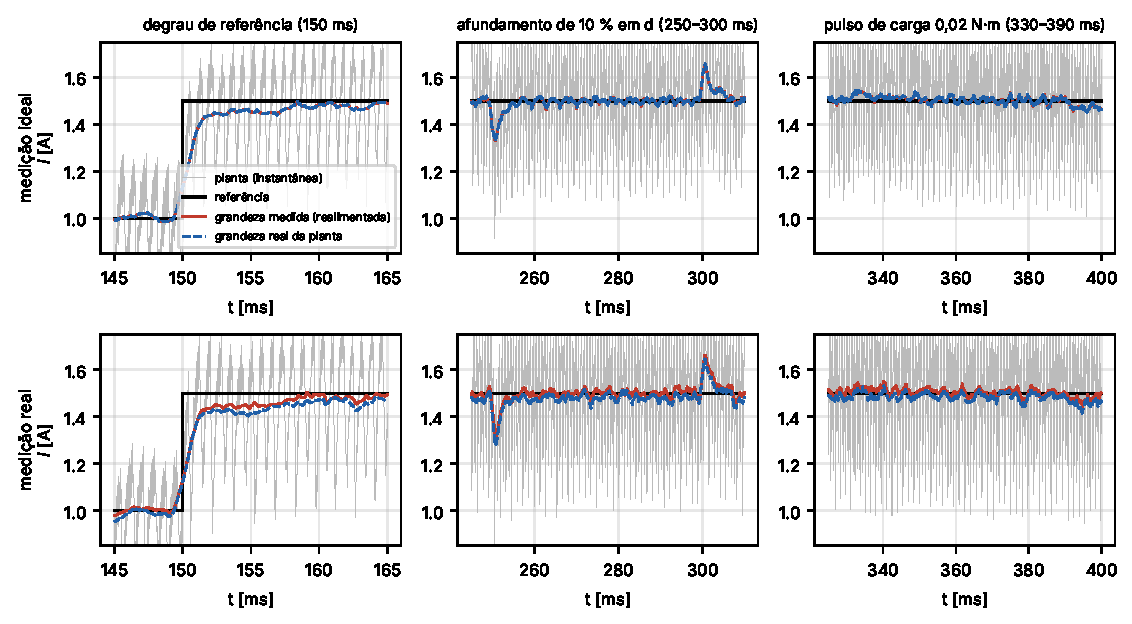
\includegraphics[width=\textwidth]{figuras/fig_r3.pdf}
\caption{Mesmo PI e mesmo ensaio, com o seletor na medição ideal (em cima, item 5) e na real (embaixo, item 6): referência, grandeza medida (realimentada), grandeza real da planta (média de 2 intervalos de comutação) e a planta instantânea (cinza).}\label{fig:r3}
\end{figure}

%======================================================================
\R{6. Controle com instrumento real}
O seletor \texttt{G07\_fb\_real} troca só a fonte da realimentação: o PI, os ganhos e a sequência são os mesmos (Fig.~\ref{fig:r3}, linha de baixo).

\begin{table}[!htbp]\centering\footnotesize
\caption{Métricas com a medição ideal e com a real (grandeza medida e grandeza real da planta). $\times$ = critério não atendido.}\label{tab:r3}
\begin{tabular}{lrrrr}\toprule
Critério & Limite & Ideal & Real: medida & Real: planta\\\midrule
\inputtab tabelas/tab_item6.tex \bottomrule
\end{tabular}
\end{table}

\textbf{Cada diferença e a característica responsável.}
\begin{itemize}
\item \textbf{Erro estacionário: 5 mA na medida, 23 mA na planta} → \emph{ruído} (\texttt{S4}) \emph{retificado pelo módulo} do processamento. O PI zera o erro \emph{da medida}. No setor em que uma fase não conduz, sua corrente é nula e a leitura é só ruído; $|n|$ tem média $\sigma\sqrt{2/\pi}$. Com $\sigma_f$ ≈ 31 mA na saída da cadeia (Tab.~\ref{tab:contr}), a média sobre os seis setores dá $0{,}455\,\sigma_f$ ≈ 14 mA; somados aos ≈5 mA da amostragem do ADC sobre a ondulação de PWM (item 8), a medida fica ≈19 mA acima da planta, e o PI reduz a corrente real. Com a malha ideal, a medida real (não realimentada) fica 20 mA acima da planta, o que confirma o mecanismo.
\item \textbf{Sobressinal de 5 para 6 \% na planta (7 \% na medida); queda de 0,17 para 0,20 A} → \emph{atraso} de 60 µs da cadeia (média por período em \texttt{P1}, retenção do ADC em \texttt{C2} e filtro RC em \texttt{C1}): a margem de fase cai de 83° para 74°.
\item \textbf{Acomodação da planta de 4,8 ms (falha)} → consequência do viés: a planta acomoda 23 mA abaixo, perto da borda da faixa de 5 \%, e um pico da ondulação de comutação sai dela. Com faixa de 10 \%, o transitório leva 0,8 ms nos três casos.
\item \textbf{Esforço igual (0,049 contra 0,047)} → a \emph{média por período} retira a ondulação de 10 kHz da realimentação; o ruído restante, vezes $K_p$, dá só ≈0,01 em $d$.
\item \textbf{Sem efeito visível}: desvio de zero, erro de sensibilidade e temperatura, porque a \emph{correção calculada} usa os valores calibrados; banda do sensor e quantização, pequenas demais.
\end{itemize}
Com os valores nominais, o instrumento real \textbf{já viola a acomodação} (4,8 ms contra 3 ms) e usa 23 dos 30 mA do erro estacionário: o mesmo controle que passa com a medição ideal falha com a real. O item 7 mostra quanto cada característica pode piorar até os outros critérios falharem também.

%======================================================================
\R{7. Ponto de ruptura}
Três características foram varridas, cada uma em quatro níveis num único ensaio de 0,5 s (o modelo troca o nível a cada 0,1 s; em cada nível há um degrau de 1,0 para 1,5 A e um afundamento). As \textbf{previsões foram registradas antes de simular} (E04 \cite{e04}):
\begin{itemize}
\item \textbf{Desvio de zero não compensado} $\delta = e_Q/S$ por fase (a fase $c$ herda $-2\delta$): a planta vai para $i^* - \tfrac23\delta$. Com 22 mA já usados pelo ruído, a folga é de 8 mA: $\tfrac23\delta \le 8$ mA ⇒ $\delta \le$ 12 mA = \textbf{1,2 mV}. Colapso quando a leitura com corrente nula, $2\delta$, passa de $i^*$ (75 mV).
\item \textbf{Filtro RC}: a corrente é alternada ($f_e$ ≈ 247 Hz com 1,5 A; o período do Hall A deu 249 Hz); o filtro atenua a leitura por $|H(f_e)| = 1/\sqrt{1+(f_e/f_c)^2}$ e a planta sobe para $i^*/|H|$. Erro de 30 mA quando $|H| = 0{,}98$: $f_c$ ≈ \textbf{1,2 kHz}.
\item \textbf{Ruído}: viés de $0{,}455\,\sigma_f$, com $\sigma_f$ proporcional a $\sigma_v$: 30 mA com $\sigma_v$ ≈ \textbf{19 mV}; esforço $K_p\sigma_f$ = 0,08 com ≈74 mV.
\end{itemize}

\begin{figure}[!htbp]\centering
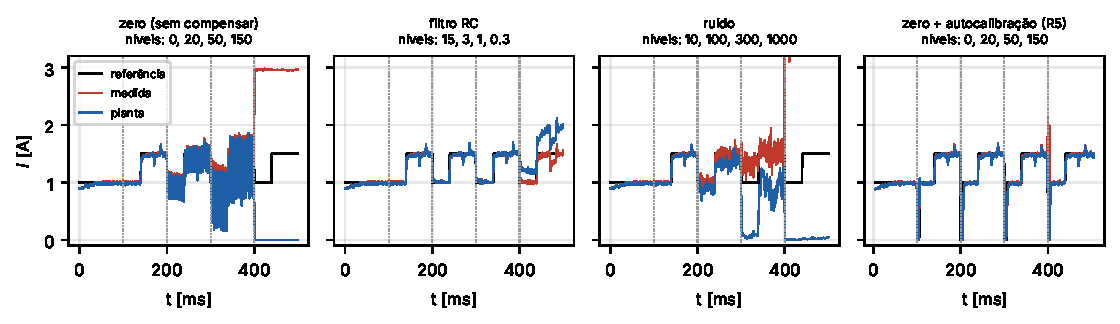
\includegraphics[width=\textwidth]{figuras/fig_varreduras.pdf}
\caption{Varreduras no VHIL (níveis trocados a cada 0,1 s, linhas pontilhadas): referência, medida e planta. As três primeiras são o item 7; a da direita é a autocalibração do item 8.}\label{fig:var}
\end{figure}

\begin{table}[!htbp]\centering\footnotesize
\caption{Previsão e resultado por nível (erro = referência $-$ planta; $\times$ = critério não atendido). O primeiro nível de cada bloco é o nominal.}\label{tab:r4}
\begin{tabular}{llrrrrrr}\toprule
Característica & Nível & Erro previsto [mA] & Erro [mA] & Sobressinal [\%] & Desvio de $d$ & Saturado [\%] & $|\Delta i|$ [A]\\\midrule
\inputtab tabelas/tab_item7.tex \bottomrule
\end{tabular}
\end{table}

\begin{figure}[!htbp]\centering
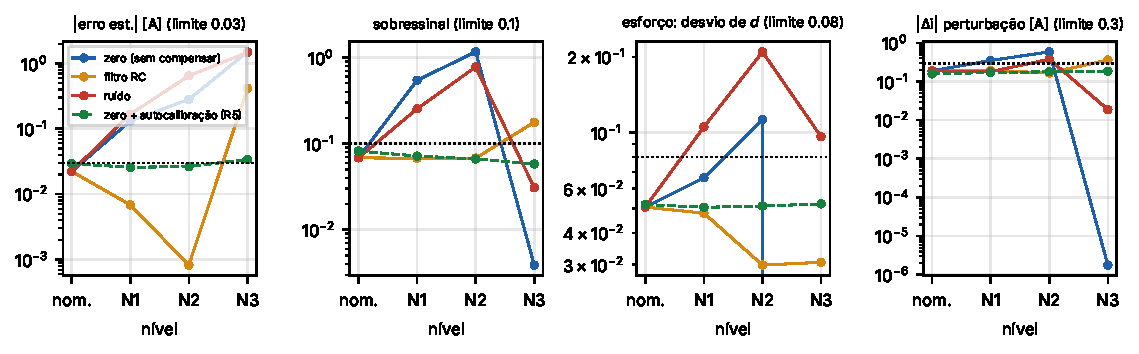
\includegraphics[width=\textwidth]{figuras/fig_mapa.pdf}
\caption{Mapa de desempenho: cada critério (linha pontilhada = limite) em função do nível de cada característica.}\label{fig:mapa}
\end{figure}

\begin{table}[!htbp]\centering\footnotesize
\caption{Pontos de ruptura: intensidade a partir da qual cada critério deixa de ser atendido (interpolação entre os níveis), contra a previsão registrada antes da simulação.}\label{tab:rup}
\begin{tabular}{lcccc}\toprule
Característica & Erro estacionário & Sobressinal & Esforço & Rejeição\\\midrule
Desvio de zero não compensado [mV] & \textbf{1,4} (prev. 1,2) & 1,3 & 29 & 14\\
Filtro RC, $f_c$ [kHz] & \textbf{0,95} (prev. 1,2) & 0,8 & não falha & 0,5\\
Ruído [mV rms] & \textbf{15} (prev. 19) & 25 & 58 (prev. 74) & 220\\\bottomrule
\end{tabular}
\end{table}

\textbf{Leitura.} Os pontos de ruptura são interpolados entre níveis distantes (0 e 20 mV; 10 e 100 mV; 1 e 0,3 kHz): a diferença de 1,2 para 1,4 mV no zero está dentro da incerteza dessa interpolação, e uma varredura fina perto do ponto (0/1/2/3 mV) daria o valor com mais precisão. O critério mais frágil é o erro estacionário, e a característica decisiva é o \textbf{desvio de zero}: 1,4 mV, menos que a própria deriva térmica do sensor entre 25 e 60 °C (2,45 mV). O \textbf{ruído} vem em seguida (15 mV, só 50 \% acima do nominal), porque o módulo o converte em viés. A banda (filtro RC) só pesa perto da frequência elétrica. As previsões erraram para o lado otimista no ruído (19 contra 15 mV) e no RC (1,2 contra 0,95 kHz): no RC, a atenuação também reduz o ruído e compensa parte do viés, o que a fórmula não considerou.

%======================================================================
\R{8. Compensação e circuitos auxiliares}
\textbf{Características escolhidas.} Aqui, como no item 3 e na Fig.~\ref{fig:f1}, \emph{circuito auxiliar} é tudo o que fica entre o sensor e o controlador: o condicionamento analógico (filtro RC), o ADC e o processamento digital (correção, média e o cálculo da grandeza controlada). O item 7 mostrou três limites estreitos; dois deles nascem nesse circuito auxiliar, fora do sensor:
\begin{enumerate}
\item a \textbf{atenuação do filtro RC} na frequência elétrica, criada pelo circuito auxiliar de condicionamento (ruptura em 0,95 kHz);
\item o \textbf{viés do ruído retificado}, criado pelo processamento (circuito auxiliar digital): o módulo transforma um erro aleatório de média nula num erro sistemático (ruptura em 15 mV);
\item o \textbf{desvio de zero}, do sensor, mas agravado pelo processamento: a fase calculada $i_c = -(i_a+i_b)$ herda o dobro do zero (ruptura em 1,4 mV).
\end{enumerate}

\textbf{Métodos do Cap.~2 e justificativa.}
\begin{itemize}
\item \textbf{(a) Filtro RC → correção calculada (2.5.3).} O efeito é conhecido em forma fechada ($|H(f_e)|$, com $f_c$ de projeto), e a frequência elétrica já está disponível no próprio acionamento: o período do sensor Hall A de posição dá $f_e$. A medida é dividida por $|H(f_e)|$ (caixa \texttt{G07\_comp\_rc}). Alternativas: um filtro inverso exato amplificaria o ruído até o limite de Nyquist (ganho de até $f_s/2f_c$ = 33 com 0,3 kHz); subir $f_c$ é mudar o projeto, não compensar.
\item \textbf{(b) Ruído retificado → insensibilidade inerente (2.5.1).} Em vez de corrigir o viés, o processamento passa a não criá-lo: os sensores Hall de posição indicam o setor e, em cada setor, usa-se com o sinal certo a fase que conduz nos dois setores vizinhos (a que carrega a corrente inteira também durante a comutação). A operação passa a ser linear, e um ruído de média nula produz erro de média nula (caixa \texttt{G07\_hall}). Alternativas: a correção calculada do viés ($0{,}455\,\sigma_f$) exigiria conhecer $\sigma_f$, que muda com a temperatura e a interferência; filtrar mais antes do módulo (2.5.2) aumentaria o atraso e reduziria a margem de fase. Custo previsto: a fase $c$ é calculada e tem o dobro da variância, então o ruído realimentado cresce ≈1,4 vez.
\item \textbf{(c) Zero → correção calculada com autocalibração (2.5.3, E04).} Ao ligar, o inversor fica 5 ms com $d$ = 0; a corrente vai a zero, o processamento média o ADC depois de 3 ms e passa a usar esse valor como zero (caixa \texttt{G07\_autocal}). Alternativas: entradas opostas (2.5.4) com um terceiro sensor, impondo $i_a+i_b+i_c = 0$; realimentação (2.5.5) com um sensor Hall de malha fechada. Ambas exigem outro componente.
\end{itemize}

\textbf{Previsões registradas antes das capturas} (22/11/2026, também no \texttt{README.md}; mantidas como foram escritas):
\begin{itemize}
\item \textbf{(a)}, com \texttt{G07\_hall} = 1: sem correção, a planta vai a 1,500 / 1,505 / 1,545 / 1,94 A nos níveis 15 / 3 / 1 / 0,3 kHz, e o erro falha a partir de 1,2 kHz. Com a correção, ≈1,50 A nos quatro níveis: o erro não falha até 0,3 kHz. O atraso do filtro não é corrigido, então o sobressinal continua falhando perto de 0,8 kHz.
\item \textbf{(b)}: a planta fica em ≈1,50 A com 10 e 100 mV, e o erro só falha quando $d$ satura (acima de 300 mV). O ruído realimentado 1,4 vez maior baixa os outros limites: sobressinal ≈19 mV (antes 25), esforço ≈37 mV (antes 58), rejeição ≈185 mV (antes 220). O limite mais exigente passa de 15 mV (erro, sistemático) para ≈19 mV (sobressinal, aleatório).
\item \textbf{Configuração final} (as duas caixas em 1, valores nominais): planta ≈1,491 A, erro ≈9 mA, o mesmo da medição ideal.
\end{itemize}

\textbf{Resultados} (capturas \texttt{final\_*}, Fig.~\ref{fig:i8} e \ref{fig:i8e}, Tab.~\ref{tab:i8} a \ref{tab:ganho}).

\begin{table}[!htbp]\centering\footnotesize
\caption{Configuração final (fase pela posição e correção do RC ligadas, valores nominais) contra as duas configurações do item 6. Planta = grandeza real.}\label{tab:fin}
\begin{tabular}{lrrrr}\toprule
Critério & Limite & Ideal & Real, módulo (item 6) & Real, fase pela posição\\\midrule
Erro estacionário [mA] & ≤ 30 & 9 & 23 & \textbf{11}\\
Acomodação [ms] & ≤ 3 & 1,4 & 4,8 $\times$ & \textbf{2,2}\\
Sobressinal [\%] & ≤ 10 & 5 & 6 & 8\\
Desvio de $d$ & ≤ 0,08 & 0,047 & 0,049 & 0,049\\
Afundamento $|\Delta i|$ [A] & ≤ 0,30 & 0,17 & 0,20 & 0,18\\\bottomrule
\end{tabular}
\end{table}

\begin{itemize}
\item \textbf{Configuração final} (Tab.~\ref{tab:fin}). A medida pela posição fica 11 mA acima da planta, contra 19 mA da medida pelo módulo na mesma captura: o PI deixa a planta 11 mA abaixo da referência (previsto ≈9 mA), e a acomodação volta a atender (2,2 ms). A seleção aplicada às correntes verdadeiras coincide com a planta (diferença média de 0,2 mA), o que confirma a tabela de setores. Os 11 mA que sobram não vêm do ruído: em malha aberta (E03), a leitura com só o ADC ligado já fica 5 mA acima da corrente no sentido do sinal dela, porque a amostragem pega a ondulação de PWM atrasada pelo sensor e pelo RC. Esse erro some na média de uma corrente alternada, mas aparece em qualquer medida que use o sinal da corrente (módulo ou seleção).
\item \textbf{Ruído} (Fig.~\ref{fig:i8e}a). A medida pela posição não retifica o ruído: com 300 mV, a medida pelo módulo fica 650 mA acima da planta e a pela posição, 22 mA. A ruptura do erro passa de \textbf{15 para 78 mV} (5 vezes). Ela não chegou aos 300 mV previstos porque, com 100 mV, a razão cíclica já começa a saturar e o PI perde a linearidade. Como previsto, o limite mais exigente passa a ser o sobressinal, que é aleatório: 17 mV (previsto 19; com o módulo, 25 mV). O esforço passou a falhar em 64 mV, e não em 37 mV como previsto: o ruído da medida pela posição ficou só 4 \% maior que o da medida pelo módulo no nível nominal (135 contra 130 mA rms), e não 1,4 vez: a fase $c$ calculada pesa menos do que a conta supôs.
\item \textbf{Filtro RC} (Fig.~\ref{fig:i8e}b). Com a fase pela posição e sem correção, a ruptura do erro fica em 0,96 kHz (igual à do item 7). A correção calculada \textbf{errou a previsão}: com 0,3 kHz, reduziu o erro de 556 para 105 mA, mas com 1 kHz o \emph{piorou} de 1 para 38 mA, e a ruptura subiu para 1,7 kHz. O motivo: $|H(f_e)|$ descreve a atenuação de uma senoide em regime, mas a medida pela posição lê cada fase só no segundo setor em que ela conduz, quando a saída do filtro já assentou, se $\tau_{RC} = 1/(2\pi f_c)$ for bem menor que um setor (0,68 ms). Com 1 kHz, $\tau_{RC}$ = 0,16 ms: não há atenuação a corrigir, e a correção só aumenta a leitura. A correção certa dependeria da forma de onda e do instante de leitura, e não só de $f_c$; por isso a recomendação para o filtro é de projeto ($f_c$ ≥ 1,2 kHz), não de compensação.
\end{itemize}

\begin{figure}[!htbp]\centering
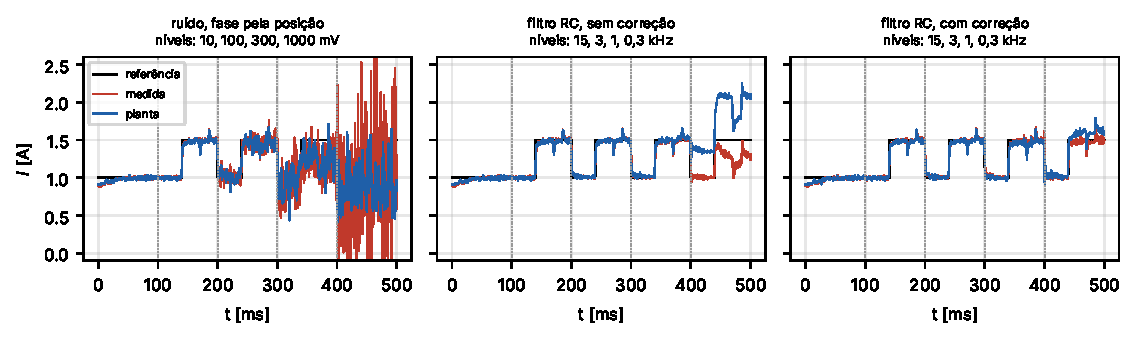
\includegraphics[width=\textwidth]{figuras/fig_item8.pdf}
\caption{Varreduras do item 8 no VHIL com a fase escolhida pela posição: ruído, filtro RC sem correção e filtro RC com a correção calculada.}\label{fig:i8}
\end{figure}

\begin{figure}[!htbp]\centering
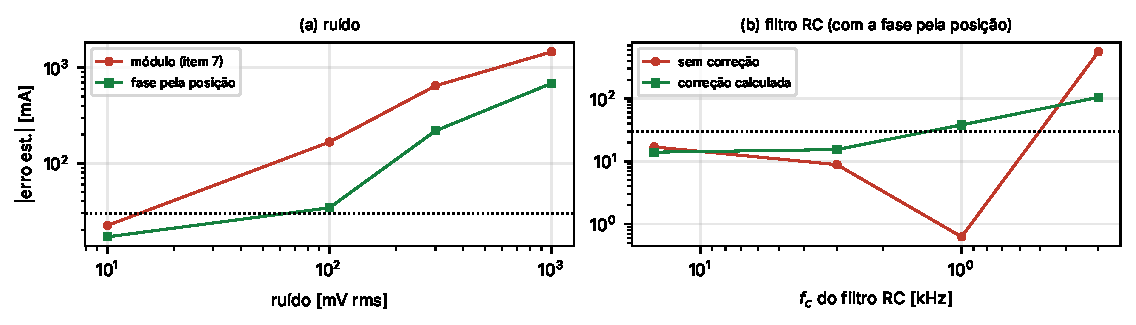
\includegraphics[width=\textwidth]{figuras/fig_item8_erro.pdf}
\caption{Erro estacionário da planta por nível (linha pontilhada = 30 mA). (a) Ruído: módulo (item 7) contra fase pela posição. (b) Filtro RC com a fase pela posição: sem e com a correção calculada.}\label{fig:i8e}
\end{figure}

\begin{table}[!htbp]\centering\footnotesize
\caption{Métricas por nível nas varreduras do item 8 ($\times$ = critério não atendido). O nível nominal das varreduras dá 14–17 mA de erro porque é medido logo após o degrau, com o motor ainda acelerando.}\label{tab:i8}
\begin{tabular}{llrrrrr}\toprule
Ensaio & Nível & Erro [mA] & Sobressinal [\%] & Desvio de $d$ & Saturado [\%] & $|\Delta i|$ [A]\\\midrule
\inputtab tabelas/tab_item8.tex \bottomrule
\end{tabular}
\end{table}

\begin{table}[!htbp]\centering\footnotesize
\caption{Ganho das compensações sobre os pontos de ruptura do erro estacionário no item 7.}\label{tab:ganho}
\begin{tabularx}{\textwidth}{p{4.1cm}p{3.9cm}ccY}\toprule
Característica & Compensação (Cap.~2) & Antes & Depois & Resultado\\\midrule
Ruído (retificado pelo processamento) & insensibilidade inerente (2.5.1) & 15 mV & \textbf{78 mV} & 5 vezes; limite global 15 → 17 mV (sobressinal)\\
Desvio de zero (dobrado em $i_c$) & autocalibração (2.5.3) & 1,4 mV & \textbf{97 mV} & 70 vezes; demais critérios passam até 150 mV\\
Filtro RC (circuito auxiliar analógico) & correção calculada (2.5.3) & 0,96 kHz & 1,7 kHz & piora; só ajuda com $f_c$ ≪ 1 kHz\\\bottomrule
\end{tabularx}
\end{table}

\textbf{Balanço do requisito.} A compensação que atende ao item 8 é a da característica criada pelo processamento (circuito auxiliar digital): a seleção pela posição multiplica por 5 a ruptura do ruído e leva o controle nominal de volta aos critérios. Para a característica do circuito auxiliar analógico, o filtro RC, nenhum método do Cap.~2 coube: a correção calculada piorou o resultado, e a solução é de projeto ($f_c$ ≥ 1,2 kHz).

\textbf{Autocalibração (resultado da E04, Fig.~\ref{fig:var} à direita).} Com zero não compensado de 0 a 50 mV, o erro fica entre 26 e 29 mA, contra 22, 132 e 282 mA sem a ação. O limite do erro sobe de 1,4 para 97 mV, e os demais critérios passam em todos os níveis. O custo é uma interrupção de torque de 5 ms em cada calibração, sem atraso nem esforço extra dentro da malha.

%======================================================================
\R{9. Síntese e reprodução}
\textbf{O que exigir deste sistema.} Em malha fechada, o controlador zera o erro \emph{da medida}: tudo o que desloca a média da leitura passa inteiro, com sinal trocado, para a corrente do motor, enquanto o que só a espalha é atenuado pela malha. Por isso as exigências são, em ordem:
\begin{itemize}
\item \textbf{Sensor.} O zero é decisivo: 1,4 mV não compensados (14 mA) já violam o erro de torque de 2 \%, e só a temperatura desloca o zero do ACS712 em 2,45 mV. Como o próprio ACS712 deriva mais que isso com a temperatura, o zero \emph{precisa} ser calibrado no sistema, com o inversor parado, ou o sensor precisa ser de outro tipo (Hall de malha fechada). O ruído deve ficar abaixo de ≈15 mV rms (≈150 mA), ou de ≈17 mV com o processamento pela posição (aí o limite passa a ser o sobressinal, não o viés); a banda de 80 kHz é 23 vezes a demanda e não limita o laço; o erro de sensibilidade de 1,5 \% vira 22 mA de erro se não for calibrado.
\item \textbf{Condicionamento.} Filtro anti-aliasing com $f_c$ ≥ 1,2 kHz, cerca de 5 vezes a frequência elétrica máxima. A correção calculada de $|H(f_e)|$ não substitui essa exigência (item 8). ADC de 12 bits basta (12 mA por degrau); a amostragem deve ser síncrona com o PWM para a ondulação de 10 kHz não virar erro.
\item \textbf{Processamento.} Correção calculada de zero, ganho e temperatura; média por período de PWM; autocalibração do zero na partida; e uma grandeza controlada que não retifique o ruído (fase escolhida pela posição em vez do módulo).
\end{itemize}

\textbf{Reprodução.} Typhoon HIL Control Center 2026.3; arquivos em \texttt{fase-2/entrega-final/simulacao/} (o \texttt{README.md} da pasta \texttt{entrega-final} explica as três subpastas): \texttt{modelo\_final.tse}, \texttt{painel\_final.cus}, \texttt{README.md}, \texttt{codigo\_c\_functions.md} e \texttt{dados-vhil/}. O README dá o bloco do \emph{Model initialization}, as caixas e o preset de cada captura, e o resultado esperado:
\begin{itemize}
\item \textbf{Item 4}: bloco A (\texttt{g07\_modo} = 1, 2 ou 3), preset \texttt{Item4\_malha\_aberta}.
\item \textbf{Itens 5 e 6}: bloco B (\texttt{g07\_modo} = 5, \texttt{g07\_cl\_ens} = 1), preset \texttt{Default}, \texttt{G07\_fb\_real} = 0 e 1.
\item \textbf{Itens 7 e 8}: bloco C (\texttt{g07\_cl\_ens} = 2, 3 ou 4), preset \texttt{R4\_varredura}, com \texttt{g07\_hall0} e \texttt{g07\_comp0} em 0 (item 7) ou 1 (item 8). A configuração final do item 8 é o bloco B com os dois em 1.
\end{itemize}

\begin{thebibliography}{9}\small
\bibitem{aguirre} L. A. Aguirre. \emph{Fundamentos de Instrumentação}. São Paulo: Pearson, 2013.
\bibitem{acs712} Allegro MicroSystems. \emph{ACS712: Fully Integrated, Hall Effect-Based Linear Current Sensor IC}, datasheet ACS712-DS.
\bibitem{moons} MOONS'. \emph{R42BLD30L3 Brushless DC Motor}, catálogo.
\bibitem{e01} G07. Caracterização da planta no domínio de origem: motor BLDC MOONS' R42BLD30L3 (Fase 2, Entrega 01). ECOM060, UFAL, 2026.
\bibitem{e02} G07. Equivalente elétrico no TyphoonSim: motor BLDC MOONS' R42BLD30L3 (Fase 2, Entrega 02). ECOM060, UFAL, 2026.
\bibitem{e03} G07. Instrumentação em malha aberta: corrente de fase do motor BLDC (Fase 2, Entrega 03). ECOM060, UFAL, 2026.
\bibitem{e04} G07. Malha fechada com instrumentação real: controle de corrente do motor BLDC (Fase 2, Entrega 04). ECOM060, UFAL, 2026.
\bibitem{ty} Typhoon HIL. Schematic Editor, HIL SCADA e Capture/Scope, documentação da versão 2026.3.
\end{thebibliography}
\end{document}
